\section{Results} \label{sec:results}
From the posteriors of galaxy properties inferred using
PROVABGS~(Section~\ref{sec:provabgs}), we derive the marginalized posteriors: 
$p(M_* \given {\bfi X_i})$, the marginalized 1D posterior of $M_*$ for galaxy
$i$.
Using these posteriors, we can estimate the SMF of BGS galaxies using
population inference in a hierarchical Bayesian 
framework~\citep[\emph{e.g.}][]{hogg2010, foreman-mackey2014, baronchelli2020}.
In other words, we infer $p(\phi\given\{{\bfi X_i}\})$, the probability
distribution of population hyperparameters $\phi$ that describe the SMF,
$\Phi(M_*; \phi)$, given the DESI observations, $\{{\bfi X_i}\}$. 
For the SMF, we use a Gaussian Mixture Model~\citep[GMM;][]{press1992, mclachlan2000}, 
which provides a highly flexible parameterization for describing population
distributions: 
\begin{equation}
    \Phi(M_*; \phi) = \sum\limits_{j=1}^{k} \mathcal{N}(M_*; \phi_j).
\end{equation} 
$k$ represents the number of Gaussian components. 
$\phi_j$ represent the mean and standard deviation of the $j^{\rm th}$ Gaussian
component of the GMM. 

We take this approach over the standard approach that use point estimates of
$M_*$ because we can correctly propagate the uncertainties in our $M_*$
measurements and more robustly estimate the $M_*$ distribution --- \emph{ie.}
SMF. 
\cite{malz2020} demonstrated in the context of inferring redshift
distributions from individual photometric redshift measurements that using
point estimates is statistically incorrect and can lead to biased redshift
distributions. 
We emphasize that \cite{malz2020} is an analogous analysis with a similar goal
of measuring a 1D galaxy property distribution. 

To infer $p(\phi\given\{{\bfi X_i}\})$, we follow the same approach described
in \cite{hahn2022}:
\begin{align}\label{eq:popinf}
p(\phi \given \{{\bfi X_i}\}) 
    =&~\frac{p(\phi)~p( \{{\bfi X_i}\} \given \phi)}{p(\{{\bfi X_i}\})}\\
    =&~\frac{p(\phi)}{p(\{{\bfi X_i}\})}\int p(\{{\bfi X_i}\} \given \{\theta_i\})~p(\{\theta_i\} \given \phi)~{\rm d}\{\theta_i\}.\\
    =&~\frac{p(\phi)}{p(\{{\bfi X_i}\})}\prod\limits_{i=1}^N\int p({\bfi X_i} \given \theta_i)~p(\theta_i \given \phi)~{\rm d}\theta_i\\
    =&~\frac{p(\phi)}{p(\{{\bfi X_i}\})}\prod\limits_{i=1}^N\int \frac{p(\theta_i \given {\bfi X_i})~p({\bfi X_i})}{p(\theta_i)}~p(\theta_i \given \phi)~{\rm d}\theta_i\\
    =&~p(\phi)\prod\limits_{i=1}^N\int \frac{p(\theta_i \given {\bfi X_i})~p(\theta_i \given \phi)}{p(\theta_i)}~{\rm d}\theta_i. 
\intertext{
    We estimate the integral using $S_i$ Monte Carlo samples from the
    individual posteriors $p(\theta_i \given {\bfi X_i})$: 
}
    \approx&~p(\phi)\prod\limits_{i=1}^N\frac{1}{S_i}\sum\limits_{j=1}^{S_i}
    \frac{p(\theta_{i,j} \given \phi)}{p(\theta_{i,j})}.
\end{align} 

%BGS provides two samples: BGS Bright and Faint. 
%Galaxies in BGS Bright are selected based on a $r < 19.5$ flux limit, while
%the ones in BGS Faint are selected based on a fiber-magnitude and color limit
%and $r < 20.0175$ flux limit. 
Since the sample of BGS galaxies is not volume-limited and complete as a
function of $M_*$, we must account for the selection effect and incompleteness
when estimating the SMF. 
To account for the selection effects of the BGS samples, we include weights
derived from $z^{\rm max}$, the maximum redshift that galaxy $i$ could be
placed and still be included in the BGS samples. 
We derive $z^{\rm max}_i$ for every galaxy using by redshifting the SED
predicted by the best-fit parameters. 
We then derive $V^{\rm max}_i$, the comoving volume out to $z^{\rm max}_i$, and
include a factor of $1/V^{\rm max}_i$ in the galaxy weight $w_i$. 

Next, we include correction weights for spectroscopic incompleteness driven by
fiber assignment and redshift failures. 
Incompletenss from fiber assignment is due to the fact that DESI is not able to
assign fibers to all galaxies included in the BGS target selection. 
Furthermore, due to galaxy clustering there is significant variation in the
assignment probability. 
Meanwhile, incompleteness from redshift failure is caused by the fact that we
do not successfully measure the redshift for every spectra and the redshift
failure rate depends on the surface brightnesses of the galaxies and the
signal-to-noise ratio of the spectra. 
We describe how we derive $w_{i, {\rm FA}}$ and $w_{i, {\rm ZF}}$, the
incompleteness correction weights for fiber assignment and redshift failures in
Appendix~\ref{sec:spec_comp}. 
Each BGS galaxy is assigned a weight of 
$w_i = (w_{i, {\rm FA}}\times w_{i, {\rm ZF}})/V^{\rm max}_i$.

We modify Eq.~\ref{eq:popinf} to include $w_i$: 
\begin{align}
p(\phi \given \{{\bfi X_i}\}) 
    \approx&~\frac{p(\phi)}{\prod\limits_{i=1}^N p({\bfi X_i})^{w_i}} 
    \prod\limits_{i=1}^N \left(\int p({\bfi X_i} \given \theta_i)~p(\theta_i \given \phi)~{\rm d}\theta_i \right)^{w_i} \\ 
    \approx&~\frac{p(\phi)}{\prod\limits_{i=1}^N p({\bfi X_i})^{w_i}} 
    \prod\limits_{i=1}^N \left( \sum\limits_{j=1}^{S_i}
    \frac{p(\theta_{i,j} \given \phi)}{p(\theta_{i,j})} \right)^{w_i} \\
    \approx&~\frac{p(\phi)}{\prod\limits_{i=1}^N p({\bfi X_i})^{w_i}} 
    \prod\limits_{i=1}^N \left( \sum\limits_{j=1}^{S_i}
    \frac{q_\phi(\theta_{i,j})}{p(\theta_{i,j})} \right)^{w_i}.
\end{align} 

In practice, we do not derive the full posterior 
$p(\phi \given \{{\bfi X_i}\})$. 
Instead we derive the maximum a posteriori (MAP) hyperparameter 
$\phi_{\rm MAP}$ that maximizes $p(\phi \given \{{\bfi X_i}\})$ or 
$\log p(\phi \given \{{\bfi X_i}\})$.
We expand, 
\begin{align}
\log p(\phi \given \{{\bfi X_i}\}) 
    \approx&~\log p(\phi) + % \sum\limits_{i=1}^N w_i \log w_i + 
    \sum\limits_{i=1}^N w_i \log \left(\sum\limits_{j=1}^{S_i} \frac{q_\phi(\theta_{i,j})}{p(\theta_{i,j})} \right).
\end{align} 
Since the first two terms are constant, we derive $\phi_{\rm MAP}$ by
maximizing 
\begin{equation}
    \max_\phi~~\sum\limits_{i=1}^N w_i \log \left(\sum\limits_{j=1}^{S_i} \frac{q_\phi(\theta_{i,j})}{p(\theta_{i,j})} \right).
\end{equation}
using the {\sc Adam} optimizer~\citep{kingma2017}.  
We derive $\phi_{\rm MAP}$ for BGS galaxies in redshift bins of width 
$\Delta z = 0.04$ starting from $z =0.01$. 
This enables us to examine the redshift evolution of the SMF within BGS. 

%\approx&~\log p(\phi) - 
%\log \prod\limits_{i=1}^N p({\bfi X_i})^{w_i} + 
%\log \prod\limits_{i=1}^N \left(\int p({\bfi X_i} \given \theta_i)~p(\theta_i \given \phi)~{\rm d}\theta_i \right)^{w_i} \\
%\approx&~\log p(\phi) - 
%\sum\limits_{i=1}^N w_i \log p({\bfi X_i}) + 
%\sum\limits_{i=1}^N w_i \log \left(\int p({\bfi X_i} \given \theta_i)~p(\theta_i \given \phi)~{\rm d}\theta_i \right) \\
%\approx&~\log p(\phi) + 
%\sum\limits_{i=1}^N w_i \log \left(\frac{1}{w_i} \sum\limits_{j=1}^{S_i} w_{i,j} \frac{p(\theta_{i,j} \given \phi)}{p(\theta_{i,j}} \right) \\

%\subsection{Targeting Completeness} \label{sec:ts}
% https://desi.lbl.gov/trac/wiki/ClusteringWG/LSScat/SV3/version2.1/fulldat
% https://desi.lbl.gov/trac/wiki/ClusteringWG/LSScat/SV3/version2.1/fullran

\begin{figure}
\begin{center}
    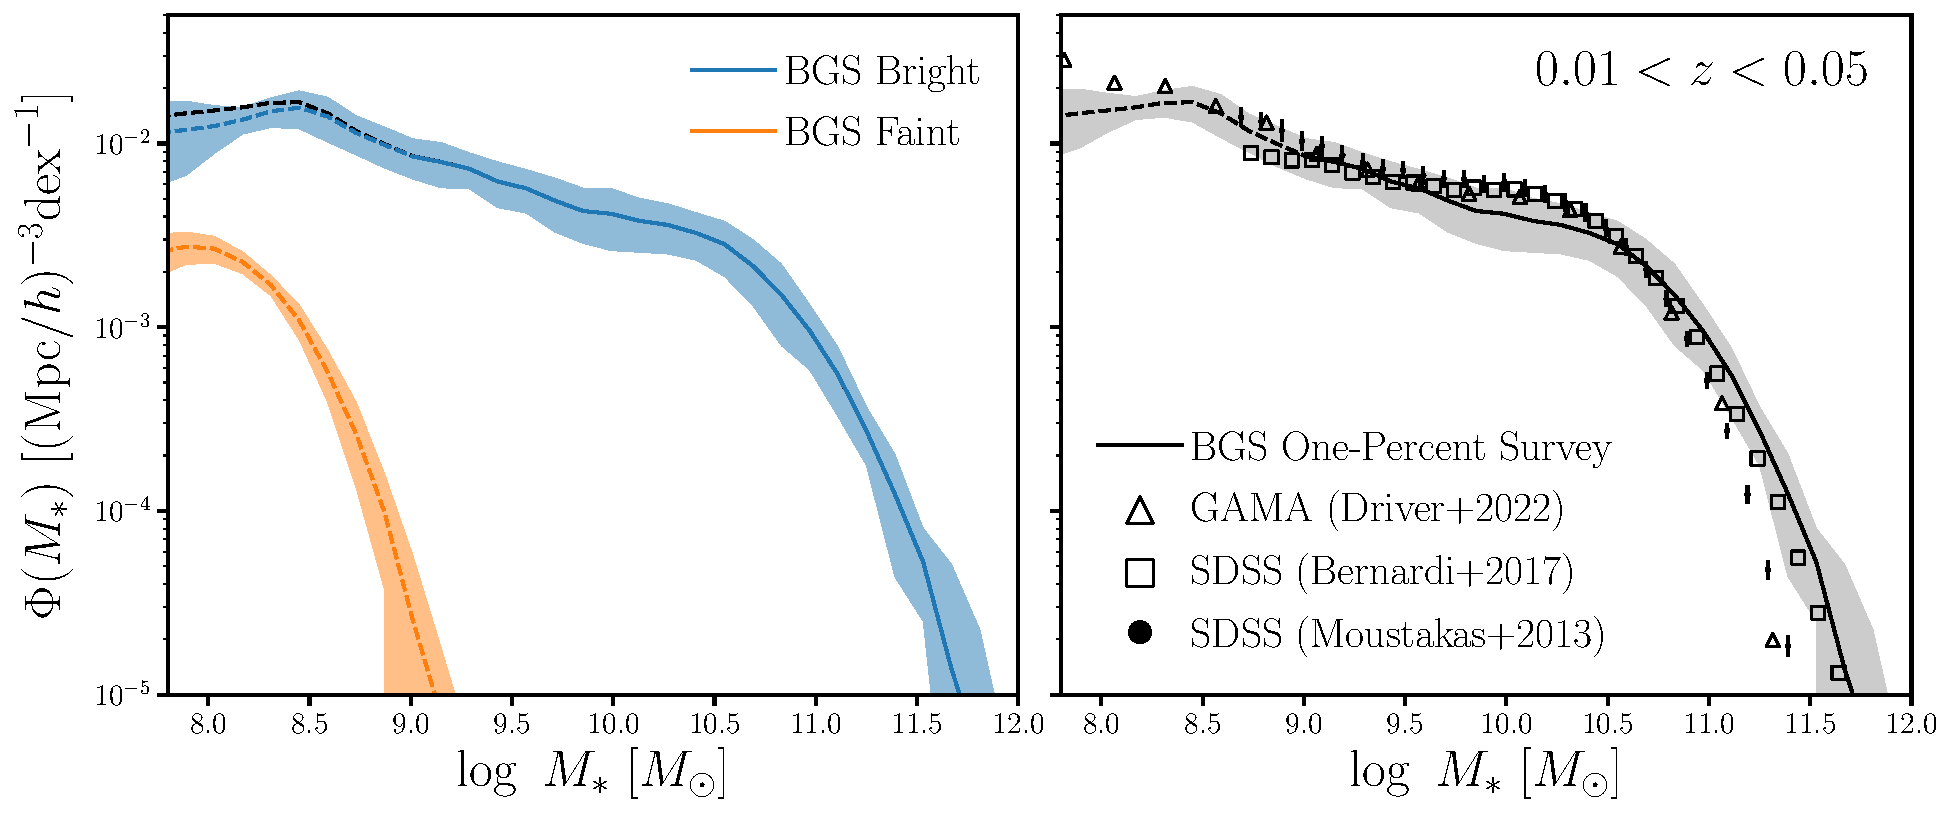
\includegraphics[width=\textwidth]{figs/psmf_bgs_any_comp.pdf} 
    \caption{
        The probabilistic SMF (pSMF) of BGS galaxies in the One-Percent Survey
        at $0.01 < z < 0.05$ (black line). 
        We represent uncertainties on the pSMF, estimated using a standard
        jackknife technique (Appendix~\ref{sec:jack}), in the shaded regions.
        The solid line represents the pSMF above the completeness limit 
        $M_* > M_{\rm lim} = 10^{8.975}M_\odot$ (Appendix~\ref{sec:mscomp}).
        In the left panel, we include SMF measurements from previous
        spectroscopic surveys for comparison: SDSS~\citep{moustakas2013,
        bernardi2017} and GAMA~\citep{driver2022}. 
        In the right panel, we present the pSMFs of BGS Bright (blue) and
        Faint (orange) galaxies. 
        Overall, the SMF of BGS are in good agreement with previous SMF
        measurements in the literature.  
    }\label{fig:psmf}
\end{center}
\end{figure}

\begin{figure}
\begin{center}
    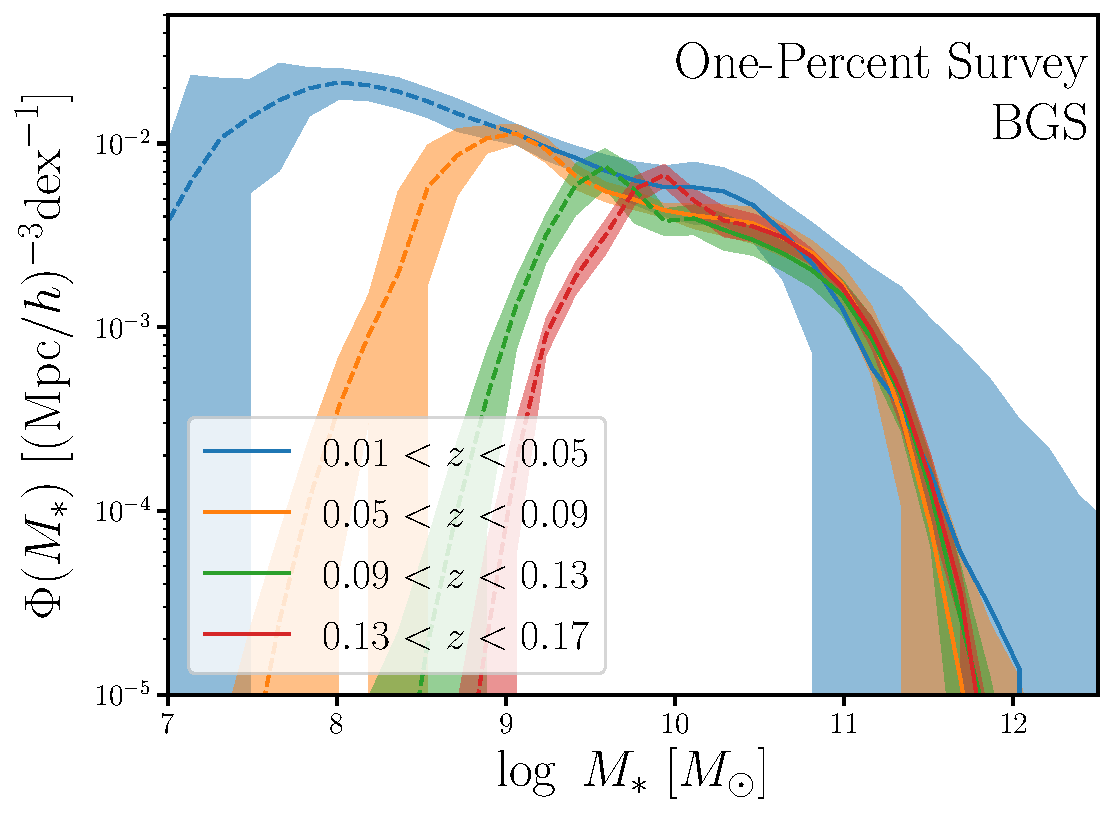
\includegraphics[width=0.6\textwidth]{figs/psmf_bgs_any_zevo.pdf} 
    \caption{
        The redshift evoution of the BGS pSMF over $0.01 < z < 0.17$. 
        The shaded regions represent the uncertainties on the pSMF, estimated
        using a standard jackknife technique.
        The solid line represents the pSMF above the completeness limit 
        $M_* > M_{\rm lim}$.
        {\color{red} takeaway message here}.
    }\label{fig:psmfz}
\end{center}
\end{figure}

\subsection{The Probabilistic Stellar Mass Function} \label{sec:psmf}
We present the probabilistic SMF (pSMF) of $0.01 < z < 0.05$ BGS galaxies in the
One-Percent Survey in Figure~\ref{fig:psmf} (blue). 
We represent the uncertainties on the SMF from sample variance in the shaded
region.
The uncertainties are estimated using a standard jackknife technique, which we
describe in Appendix~\ref{sec:uncert} (Eq.~\ref{eq:jack}) and provide
conservative estimates~\citep{norberg2009}. 
In the right panel, we present the pSMFs of galaxies in the BGS Bright and
Faint galaxies.  

In the left panel, we include SMF measurements from previous spectroscopic 
surveys SDSS~\citep{moustakas2013, bernard2017} (black circle and square) and
GAMA~\citep{driver2022} (black triangle) for comparison.
\todo{mention the correction in driver}
Overall, we find good agreement with previous SMF measurements. 

In Figure~\ref{fig:psmfz}, we present the redshift evolution of the pSMF 
